\documentclass{article}

\usepackage[utf8]{inputenc}
\usepackage{enumitem}
\usepackage{amsmath}
\usepackage{amsthm}
\usepackage{amssymb}
\usepackage{graphicx}
\usepackage{tikz}
\usepackage[normalem]{ulem}

\newcommand{\mname}[1]{\mbox{\sf #1}}
\newcommand{\pnote}[1]{{\langle \text{#1} \rangle}}

\newcommand{\GETS}{:=}

%% Highlight, strike-out
\newcommand{\key}[1]{\underline{\smash{#1}}}
\newcommand{\pkey}[1]{\dashuline{\smash{#1}}}

%% SQL
\newcommand{\SQL}[1]{\texttt{#1}}
\newcommand{\SQLK}[1]{\texttt{\bf #1}}
\newcommand{\SQLCOMMENT}{\texttt{-}\texttt{-} }

%% RA
\newcommand{\rename}{\rho}
\newcommand{\select}{\sigma}
\newcommand{\join}{\times}
\newcommand{\rel}[1]{\text{#1}}
\newcommand{\attr}[1]{\text{#1}}
\newcommand{\ra}[2]{\rel{#1}.\attr{#2}}
\newcommand{\project}{\pi}
\newcommand{\product}{\times}
\newcommand{\union}{\cup}
\newcommand{\intersect}{\cap}
\newcommand{\difference}{\setminus}
\newcommand{\goesto}[2]{#1 \mapsto #2}
\newcommand{\njoin}{\Join}
\newcommand{\dedup}{\delta}
\newcommand{\group}{\gamma}

\title{Assignment 4: The Relational Algebra}
\author{Hien Tu - tun1}
\date{\today}

\begin{document}

\maketitle

\textbf{The requested queries}
\begin{enumerate}
  \item $\select_{\attr{startdate } < \attr{ enddate}}(\rel{event})$ \\
  \item $\project_{\ra{U}{uid}, \ra{E}{eid}}
          (\rename_{\rel{U}}(\rel{user}) \Join_{\ra{U}{postcode } = \ra{ E}{postcode }}
          \rename_{\rel{E}}(\rel{event}))$ \\
  \item $X \GETS
          \rename_{\rel{E}}(\rel{event}) \Join_{\ra{E}{eid } = \ra{ EnoRv}{eid}}
          \rename_{\rel{EnoRv}}
            (\project_{\attr{eid}}(\rel{event}) \difference
            \project_{\attr{event}}(\rel{review}))$ \\
        $\project_{\ra{E}{eid}, \ra{E}{title}, \ra{E}{description},
          \ra{E}{startdate}, \ra{E}{enddate}, \ra{E}{organizer},
          \ra{E}{postcode}}(X)$ \\
  \item Select events with at least 3 keywords: \\
        $X \GETS \rename_{\rel{K}_1}(\attr{keyword}) \product
                  \rename_{\rel{K}_2}(\attr{keyword}) \product
                  \rename_{\rel{K}_3}(\attr{keyword})$ \\
        $Y \GETS \select_{K_1.\attr{word } \neq K_2.\attr{ word } \land
                          K_1.\attr{word } \neq K_3.\attr{ word } \land
                          K_2.\attr{word } \neq K_3.\attr{ word }}(X)$ \\
        $Z \GETS \select_{K_1.\attr{event } = K_2.\attr{event } \land
                          K_1.\attr{event } = K_3.\attr{event }}(Y)$ \\ \\
        Select events with at least 2 keywords: \\
        $A \GETS \rename_{\rel{K}_4}(\attr{keyword}) \product
                  \rename_{\rel{K}_4}(\attr{keyword})$ \\
        $B \GETS \select_{K_4.\attr{word } \neq K_5.\attr{word}}(A)$ \\
        $C \GETS \select_{K_4.\attr{event } = K_5.\attr{event}}(B)$ \\ \\
        Select events with exactly 3 keywords: \\
        $\project_{K_4.event}(C) \difference \project_{K_1.event}(Z)$ \\
  \item
    \begin{enumerate}
      \item $X \GETS \rename_{R_1}(\rel{review}) \product
                      \rename_{R_2}(\rel{review})$ \\ \\
            Keep reviews from $R_1$ that are not from latest date: \\
            $Y \GETS \select_{R_1.\attr{reviewdate } < R_2.\attr{reviewdate }
                              \land R_1.\attr{user } = R_2.\attr{user }}(X)$ \\ \\
            Select user id and event id for which the user wrote a review most
            recently: \\
            $Z \GETS
              \project_{\attr{user}, \attr{event}}(\rel{review}) \difference
              \project_{R_1.\attr{user}, R_1.\attr{event}}(Y)$ \\
      \item $A \GETS \rename_{R_1}(\rel{review}) \product
                      \rename_{R_2}(\rel{review}) \product
                      \rename_{E_1}(\rel{event}) \product
                      \rename_{E_2}(\rel{event})$ \\
            $B \GETS \select_{R_1.\attr{user } = R_2.\attr{user } \land
                              R_1.\attr{event } = E_1.\attr{eid } \land
                              R_2.\attr{event } = E_2.\attr{eid }}(A)$ \\ \\
            Select reviews whose $E_1.\attr{enddate}$ are not from the latest: \\
            $C \GETS \select_{E_1.\attr{enddate} < E_2.\attr{enddate}(B)}$ \\ \\
            Select user id and event id of the most-recent event (according to
            enddate) for which the user wrote a review: \\
            $D \GETS \project_{R_1.\attr{user}, E_1.\attr{eid}}(B \difference C)$ \\
      \item $\project_{\ra{LR}{user}, \ra{LR}{lreview}, \ra{LE}{levent}}
              (\rename_{\rel{LR}(\rel{user}, \rel{lreview})}(Z)
                \njoin_{\ra{LR}{user } = \ra{LE}{user}}
                \rename_{\rel{LE}(\rel{user}, \rel{levent})}(D))$ \\
    \end{enumerate}

\end{enumerate}


\textbf{Effiency of queries}
\begin{enumerate}
  \setcounter{enumi}{6}
  \item \ \\
    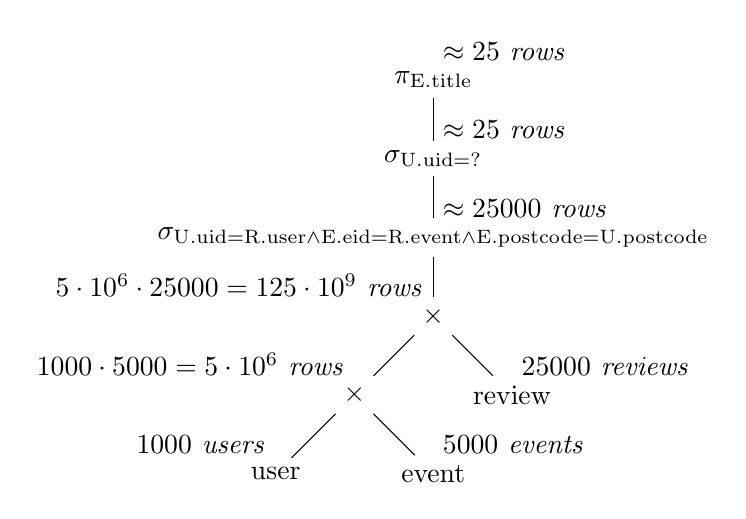
\begin{tikzpicture}
      \node (p) at (0, 0) {$\project_{\ra{E}{title}}$};
      \node[above right] at (p) {\strut{}\emph{$\approx 25$ rows}};
      \node (su) at (0, -1) {$\select_{\ra{U}{uid} = ?}$} edge (p);
      \node[above right] at (su) {\strut{}\emph{$\approx 25$ rows}};
      \node (ss) at (0, -2) {$\select_{\ra{U}{uid} = \ra{R}{user} \land \ra{E}{eid} = \ra{R}{event} \land \ra{E}{postcode} = \ra{U}{postcode}}$} edge (su);
      \node[above right] at (ss) {\strut{}\emph{$\approx 25000$ rows}};
      \node (uer) at (0, -3) {$\product$} edge (ss);
      \node[above left] at (uer) {\strut{}\emph{$5 \cdot 10^6 \cdot 25000 = 125 \cdot 10^9$ rows}};
      \node (rv) at (1, -4) {$\rel{review}$} edge (uer);
      \node[above right] at (rv) {\strut{}\emph{$25000$ reviews}};
      \node (ue) at (-1, -4) {$\product$} edge (uer);
      \node[above left] at (ue) {\strut{}\emph{$1000 \cdot 5000 = 5 \cdot 10^6$ rows}};
      \node (u) at (-2, -5) {$\rel{user}$} edge (ue);
      \node[above left] at (u) {\strut{}\emph{$1000$ users}};
      \node (e) at (0, -5) {$\rel{event}$} edge (ue);
      \node[above right] at (e) {\strut{}\emph{$5000$ events}};
    \end{tikzpicture}
\end{enumerate}

\end{document}